% c09 —— §4 矩阵模型；§4.1 Wick 定理及其变分（原书 p.64–67）
% 负责：trans-e

% ===== 原书 p.64 =====
\section{矩阵模型}

\subsection{Wick 定理及其变分}

\transnote{原书本小节标题印作「Wich」，通行为「Wick」，译本标题与正文统一作 Wick。}

本章讲述物理学中常用的 Wick 定理以及与 Feynman 图有关的微扰论。先叙述单变量的 Wick 定理。设$\kappa>0$。对多项式$f(x)\in\C[x]$，定义
\[
\langle f(x)\rangle=\int_\infty^\infty f(x)\exp(-\kappa x^2/2)\,dx.
\]
这可以看作关于 Gaussian 测度的$f(x)$的期望值。要知道$\langle f(x)\rangle$的值，知道$\langle x^i\rangle$（$i=0,1,\dots$）就够了；为此知道其指数型母函数
\[
\langle e^{jx}\rangle=\sum_{i=0}^\infty\langle x^i\rangle\frac{j^i}{i!}
\]
就够了。实际上由此可由$((\partial/\partial j)^i\langle e^{jx}\rangle)|_{j=0}$求出$\langle x^i\rangle$。$\langle e^{jx}\rangle$如下求出：
\[
\begin{aligned}
\langle e^{jx}\rangle
&=\int_\infty^\infty\exp\Bigl(-\frac{\kappa x^2}{2}+jx\Bigr)\,dx\\
&=\int_\infty^\infty\exp\Bigl(-\frac{\kappa}{2}\Bigl(x+\frac{j}{\kappa}\Bigr)^2\Bigr)\,dx
\cdot\exp\Bigl(\frac{j^2}{2\kappa}\Bigr)\\
&=\langle 1\rangle\cdot\exp\Bigl(\frac{j^2}{2\kappa}\Bigr).
\end{aligned}
\]

\transnote{原书此处的积分上下限都印作$\infty$，下限缺负号。译本照原文印出。}

其次，一般地，当写成
\[
\Bigl(\frac{\partial}{\partial j}\Bigr)^k e^{\frac12 j^2}
=\Bigl(\sum_{l=0}^k a_{kl}j^l\Bigr)e^{\frac12 j^2}
\]
时，$a_{kl}$等于准备编号$1\sim k$的顶点、再按下列规则给它们加边的方法数：
\begin{itemize}[leftmargin=3.6em,itemsep=2pt,topsep=4pt]
\item[$(R_{kl})$] 连接两个顶点的「闭边（closed edge）」有$(k-l)/2$条，其余是只连在一个顶点上的「开边（open edge）」，有$l$条。
\end{itemize}

\begin{center}
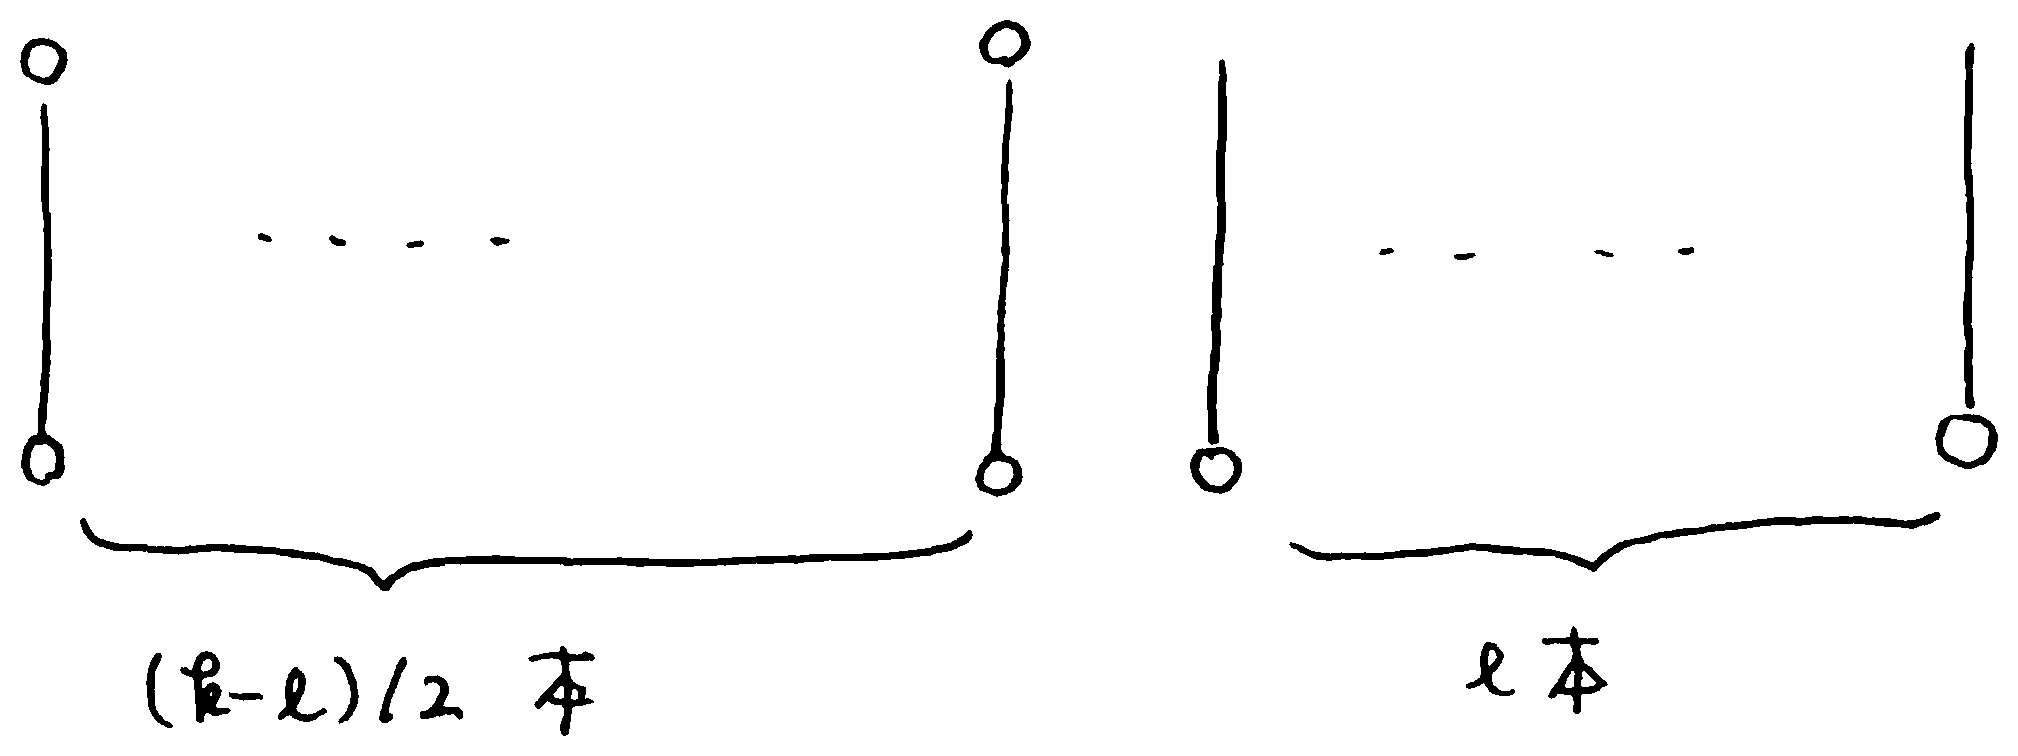
\includegraphics[width=0.60\linewidth]{fig_p70_a.png}
\end{center}

% ===== 原书 p.65 =====
实际上这可由归纳法证明。
\[
\begin{aligned}
\Bigl(\frac{\partial}{\partial j}\Bigr)^{k+1}e^{\frac12 j^2}
&=\Bigl\{\frac{\partial}{\partial j}\Bigl(\sum_{l=0}^k a_{kl}j^l\Bigr)
+\Bigl(\sum_{l=0}^k a_{kl}j^l\Bigr)\cdot j\Bigr\}e^{\frac12 j^2}\\
&=\Bigl(\sum_{l=0}^k a_{kl}\,l\,j^{l-1}
+\sum_{l=0}^k a_{kl}j^{l+1}\Bigr)e^{\frac12 j^2}
\end{aligned}
\]
成立，故只需证明$a_{k+1,l}=(l+1)a_{k,l+1}+a_{k,l-1}$即可。第一项是第$(k+1)$个顶点成为闭边的情形数，第二项是成为开边的情形。又，用此$a_{kl}$，经简单的 scale 变换得
\[
\Bigl(\frac{\partial}{\partial j}\Bigr)^k e^{j^2/(2\kappa)}
=\Bigl(\sum_{l=0}^k a_{kl}j^l\kappa^{-(k+l)/2}\Bigr)e^{j^2/(2\kappa)}.
\]
这里令$l=0$，即得下述定理。

\begin{theorem}[Wick]
\[
\frac{\langle x^k\rangle}{\langle 1\rangle}=a_{k,0}\kappa^{-k/2}.
\]
\end{theorem}

其中$a_{k0}$是把编号$1\sim k$的顶点两两配对、不剩余地全部连接起来的方法数。

这是使用 Feynman 图时的基本定理。它有许多 version，下面考虑顶点着色的版本。

设$x={}^t(x_1,\dots,x_r)$为$r$维列向量，$Q=(q_{ij})$为可逆对称矩阵。对$I=(a_1,\dots,a_r)\in\N^r$、$|a|=\sum_{i=1}^r a_i$，记$x^I=x_1^{a_1}\cdots x_r^{a_r}$。考虑求
\[
\langle x^I\rangle=\int_{\R^r}x^I\exp\Bigl(-\frac12{}^tXQX\Bigr)\,dx_1\cdots dx_r
\]
的值。设$J={}^t(y_1,\dots,y_r)$。因
\[
-\frac12{}^tXQX+{}^tJX
=-\frac12{}^t(X+Q^{-1}J)Q(X+Q^{-1}J)+\frac12{}^tJQ^{-1}J,
\]
故令$P=Q^{-1}=(p_{ij})$、$\partial^{|I|}/\partial y^I
=(\partial/\partial y_1)^{a_1}\cdots(\partial/\partial y_r)^{a_r}$，则
\[
\begin{aligned}
\langle x^I\rangle
&=\frac{\partial^{|I|}}{\partial y^I}
\int\exp\Bigl(-\frac12{}^tXQX+{}^tJX\Bigr)\,dX\Big|_{J=0}\\
&=\langle 1\rangle
\Bigl(\frac{\partial^{|I|}}{\partial y^I}\exp\Bigl(\frac12{}^tJPJ\Bigr)\Big|_{J=0}\Bigr).
\end{aligned}
\]

% ===== 原书 p.66 =====
其次，取$K=(b_1,\dots,b_r)\in\N^r$，则$(\partial^{|I|}/\partial y^I)\exp(\frac12{}^tJPJ)$中$y^K\exp(\frac12{}^tJPJ)$的系数$a_{IK}$如下计算。先准备颜色$1\sim r$。设$|I|=l$、$|K|=m$，准备$l$个 type I 的顶点并编上$1\sim l$的号。准备$m$个 type II 的顶点，不给它们编号（type II 看作前例中开边虚拟连接的对方）。把这$(l+m)$个顶点两个一组用边连接，考虑连接方式；其中不允许 type II 之间相连的情形，其余连接方式都考虑。进而给 type I、type II 的顶点涂上$1\sim r$的颜色，使 type I 中各种颜色的个数为$a_1,\dots,a_r$，type II 中各种颜色的个数为$b_1,\dots,b_r$。这样得到的着色图全体记作$\Gamma$。对$G\in\Gamma$，定义$G$的权为$w(G)=\prod_{e\in G}p_e$。这里，对$G$的边$e$，若其两端点的颜色为$s_1,s_2$，则定义$p_e=p_{s_1,s_2}$。此时下述定理成立。

\begin{theorem}[Wick 定理的着色版本]
\[
a_{IK}=\sum_{G\in\Gamma}w(G).
\]
\end{theorem}

特别地，当$K=0$时，令
\[
\Gamma_I=\left\{\begin{array}{l}
\text{将 $|I|$ 个带编号的顶点 $1,\dots,l$ 涂上颜色 $1,\dots,r$，使各颜色的个数为 $a_1,\dots,a_r$，}\\[2pt]
\text{并把它们两个一组、不剩余地用边连接成的图形}
\end{array}\right\},
\]
则
\[
\frac{\langle x^I\rangle}{\langle 1\rangle}=a_{I,0}=\sum_{G\in\Gamma_I}w(G)
\]
给出。

下面转向矩阵模型。把上述想法应用于$n\times n$ Hermitian 矩阵全体所成的向量空间$H_n$，以及其上的二次形式$Q(X)=\frac12\tr(X\Lambda X)$（$X\in H_n$）。其中$\Lambda=\operatorname{diag}(\lambda_1,\dots,\lambda_n)$（$\lambda_i\in\R_+$）。令$X=(x_{ij})$，则
\[
Q(X)=\frac12\sum_{i,j}\frac{\lambda_i+\lambda_j}{2}|x_{ij}|^2.
\]

% ===== 原书 p.67 =====
这里，把$x_{ij}$（$i\neq j$）看作复变量，则$x_{ij}=\bar{x}_{ji}$。把$x_{ii}$看作实变量。$H_n$上的测度$dX$定义为$dX=\prod_{i,j}dx_{ij}$。对$I=(i_1,\dots,i_k)$、$J=(j_1,\dots,j_k)$，置$x_{IJ}=x_{i_1j_1}\cdots x_{i_kj_k}$。考虑求
\[
\langle x_{IJ}\rangle=\int x_{IJ}\exp\Bigl(-\frac12\tr(X\Lambda X)\Bigr)\,dX
\]
的值。与前面的论述同样，
\[
\langle x_{IJ}\rangle
=\frac{\partial^k}{\partial y_{IJ}}\exp\Bigl(-\frac12\tr(J\Lambda^{-1}J)\Bigr)\Big|_{J=0}
\]
给出。

\transnote{上式右端照原文印出：指数中为$-\frac12\tr(J\Lambda^{-1}J)$，且右端没有因子$\langle1\rangle$。这与前页相应公式的符号及写法都不一致，疑为原书排印之误。}

这里取$J=(y_{ij})\in H_n\cong\C^{n(n-1)/2}\times\R^n$的坐标$y_{ij}\in\C$（$i<j$）、$y_{ii}\in\R$，看作$n(n-1)/2$个复变量、$n$个实变量的函数。按着色版本时的表示法，准备$(i,j)$（$i,j=1,\dots,n$）这$n^2$个颜色即可；而由二次形式$Q(X)$确定的对称矩阵的逆矩阵$P=(P_{(ij),(i'j')})$为
\[
p_{(i,i),(i,i)}=\frac{1}{\lambda_i},\qquad
p_{(i,j),(j,i)}=\frac{2}{\lambda_i+\lambda_j},\qquad(i\neq j),
\]
其余成分为$0$。

\transnote{此式左端原书印作小写$p$，与上一句所定义的矩阵$P$大小写不一致。译本照原文印出。}

由此，用图表示时，可以不给顶点涂$(i,j)$色，而对每个顶点给以下这样的着色箭头。

\begin{center}
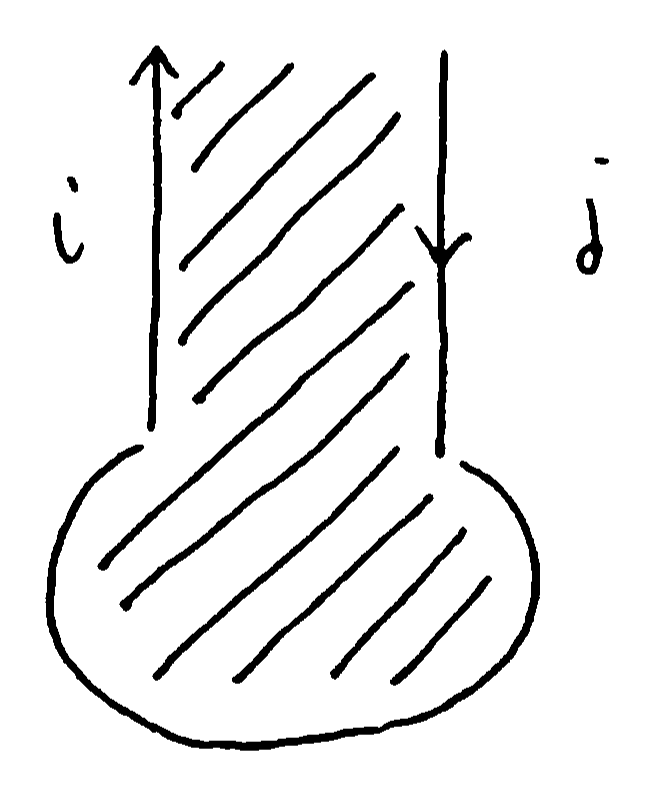
\includegraphics[width=0.26\linewidth]{fig_p73_a.png}
\end{center}

当然，考虑给顶点编号时，也对应于考虑带有上述着色箭头并且已编号的顶点。

\begin{center}
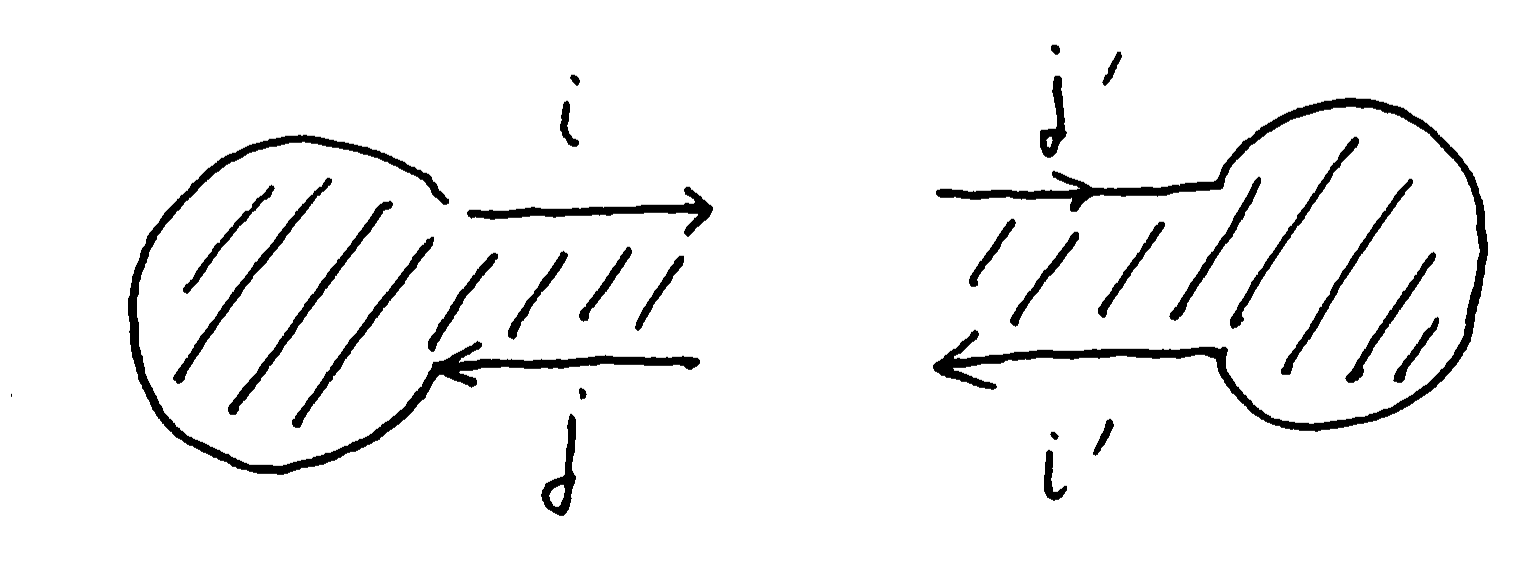
\includegraphics[width=0.62\linewidth]{fig_p73_b.png}
\end{center}
